\documentclass[12pt]{beamer}
\usetheme{CambridgeUS}
\usepackage[utf8]{inputenc}
\usepackage[spanish]{babel}
\usepackage{amsmath}
\usepackage{amsfonts}
\usepackage{amssymb}
\usepackage{graphicx}
\usepackage{ragged2e}
\setbeamertemplate{navigation symbols}{} 
\author[Kevin García - Alejandro Vargas]{Kevin García 1533173 \newline Alejandro Vargas 1525953}
\title[Análisis de componentes principales]{Laboratorio 1: Análisis de componentes principales}


\newcommand\Wider[2][3em]{%
\makebox[\linewidth][c]{%
  \begin{minipage}{\dimexpr\textwidth+#1\relax}
  \raggedright#2
  \end{minipage}%
  }%
}


%\setbeamercovered{transparent} 
%\setbeamertemplate{navigation symbols}{} 
%\logo{} 
%\institute{} 
%\date{} 
%\subject{} 
\begin{document}
\justify
\begin{frame}
\titlepage
\end{frame}

%\begin{frame}
%\tableofcontents
%\end{frame}
\begin{frame}
\frametitle{Introducción}
~\\En esta presentación veremos el uso y aplicación del análisis de componentes principales en una base de datos que contiene las importaciones hechas por los países suramericanos (Colombia, Brasil, Chile, Argentina, Ecuador y Perú), éstas provenientes de Estados Unidos, entre 1991 y 2010. Se analizará la cantidad de ejes o componentes principales a utilizar y se darán algunas interpretaciones de algunas tablas y gráficas obtenidas y de las trayectorias que se pueden formar entre los años consecutivos. Además, se analizará la posibilidad de construir un indice dependiendo de las componentes principales que obtengamos, si se da la posibilidad, se mostrará el proceso de construcción del indice y un posible re-escalamiento de este. 
\end{frame}

\begin{frame}
\frametitle{Base de datos}
\begin{center}
\resizebox{8cm}{!}{
\begin{tabular}{|ccccccc|}
\hline
Año	& Colombia & Brasil & Chile & Argentina &	Ecuador &	Peru \\
\hline
1991 &	44.4	&27.2&	45.6&	20.0&	6.0	&14.1\\
1992 &	75.5&	11.8&	58.9&	22.6&	17.8&	14.4\\
1993 &	110.7&	50.6&	128.3&	17.2&	119.4&	118.5\\
1994 &	80.3&	70.6&	102.2&	15.2&	154.9&	146.1\\
1995 &	81.6&	82.3&	89.0&	35.1&	169.4&	127.1\\
1996 &	76.4&	97.4&	185.0&	51.0&	75.5&	129.0\\
1997 &	32.0&	89.5&	195.3&	31.1&	33.4&	110.2\\
1998 &	55.5&	63.1&	66.3&	24.4&	9.7	&     66.7\\
1999 &	74.3&	72.6&	76.3&	28.1&	11.2&	110.7\\
2000 &	84.5&	76.2&	80.1&	29.5&	11.8&	110.2\\
2001 &	87.1&	97.4&	89.3&	51.5&	63.1&	89.3\\
2002 &	89.3&	89.5&	72.4&	40.3&	66.3&	70.2\\
2003 &	70.2&	63.1&	80.1&	60.5&	76.3&	90.1\\
2004 &	90.1&	66.3&	70.5&	39.1&	20.0&	64.5\\
2005 &	60.5&	76.3&	107.2&	31.1&	63.4&	92.7\\
2006 &	140.3&	20.0&	63.4&	50.2&	101.2&	120.8\\
2007 &	120.4&	22.6&	101.2&	51.0&	103.1&	107.2\\
2008 &	130.2&	17.2&	103.1&	42.5&	66.7	&70.8\\
2009 &	110.1&	31.1&	75.6&	25.7&	110.7	&101.2\\
2010 &	120.2&	24.4&	68.9&	60.3&	110.2	&110.8\\
\hline
\end{tabular}
}
\end{center}
\end{frame}

\begin{frame}
\frametitle{Estadísticas descriptivas}
~\\En la siguiente tabla se resumen las estadísticas descriptivas para las variables (los países):
\begin{center}
\resizebox{12cm}{!}{
\begin{tabular}{ccccccc}
\hline 
Descriptivas & Colombia & Brasil & Chile & Argentina & Ecuador & Perú \\ 
\hline 
Minimo & 32 & 11.8 & 45.6 & 15.2 & 6 & 14.1 \\  
1st. Cuartil & 73.28 & 26.5 & 70.1 & 25.38 & 19.45 & 70.65 \\ 
Mediana & 83.05 & 64.7 & 80.1 & 33.1 & 66.5 & 104.2 \\ 
Media & 86.68 & 57.46 & 92.94 & 36.32 & 69.5 & 93.23 \\ 
3rd. Cuartil & 110.25 & 77.8 & 102.42 & 50.4 & 104.88 & 112.72 \\ 
Máximo & 140.3 & 97.4 & 195.3 & 60.5 & 169.4 & 146.1 \\ 
Desviación Est. & 28.41033 & 29.18638 & 38.44684 & 14.08006 & 49.30692 & 34.89316 \\ 
\hline 
\end{tabular}
}
\end{center}
\end{frame}

\begin{frame}
\frametitle{ACP para los individuos $R^6$}
~\\Para llevar a cabo el análisis de componentes principales de la base de datos anterior, estandarizaremos las variables que en nuestro caso son los países, ya que aunque todas están medidas en la misma escala, podría haber diferencias por el tipo de economía que maneja cada país. La matriz de correlaciones correspondiente a esta base de datos es:

\begin{center}
\resizebox{12cm}{!}{
\begin{tabular}{|c|cccccc|}
\hline 
 & Colombia & Brasil & Chile & Argentina & Ecuador  & Perú \\
\hline  
Colombia & 1 & -0.524830476 & -0.22431855 & 0.391517899 & 0.48620724 & 0.2790988 \\ 
Brasil & -0.524830476 & 1 & 0.46610474 & 0.005930606 & -0.04478948 & 0.3709440 \\ 
Chile & -0.22431855 & 0.46610474 & 1 & 0.051451487 & 0.15920217 & 0.4937184 \\ 
Argentina & 0.391517899 & 0.005930606 & 0.05145149 & 1 & 0.16157351 & 0.1828657 \\ 
Ecuador & 0.4862072 & -0.04478948 & 0.15920217 & 0.16157351 & 1 & 0.6547563 \\ 
Perú & 0.2790988 & 0.3709440 & 0.4937184 & 0.1828657 & 0.6547563 & 1 \\ 
\hline 
\end{tabular} 
}
\end{center}
\end{frame}

\begin{frame}
\frametitle{ACP para los individuos $R^6$}
~\\Para realizar el análisis de forma multivariada, debemos diagonalizar la matriz de correlaciones, es decir, obtener su descomposición en valores y  vectores propios correspondientes.

~\\Esta matriz de correlaciones tiene 6 valores propios positivos, que son:
$$\lambda_1=2.1934092$$
$$\lambda_2=1.9561781$$
$$\lambda_3=0.9038789$$
$$\lambda_4=0.5119470$$
$$\lambda_5=0.2854407$$
$$\lambda_6=0.1491461$$
\end{frame}

\begin{frame}
\frametitle{ACP para los individuos $R^6$}
~\\Con los valores propios obtenidos, procedemos a hallar los vectores propios correspondientes

\begin{center}
\resizebox{12cm}{!}{
\begin{tabular}{|cccccc|}
\hline 
$\lambda_{1}$ & $\lambda_{2}$ & $\lambda_{3}$ & $\lambda_{4}$ & $\lambda_{5}$ & $\lambda_{6}$ \\ 
-0.3266572 & 0.5708984 & 0.0068014 & 0.1170875 & 0.5332445 & 0.5189071 \\ 
-0.1588587 & -0.6033277 & 0.2009878 & -0.5413708 & 0.1852719 & 0.4929051 \\ 
-0.3381710 & -0.4635960 & 0.0514265 & 0.7890499 & -0.0779079 & 0.1985066 \\ 
-0.2898593 & 0.2066273 & 0.8863988 & -0.0448699 & -0.2455986 & -0.1589085 \\ 
-0.5459391 & 0.1756044 & -0.3785943 & -0.2216216 & -0.6626128 & 0.1990175 \\ 
-0.6096157 & -0.1470297 & -0.1669623 & -0.1395665 & 0.4193810 & -0.6192861 \\ 
\hline 
\end{tabular} 
}
\end{center}
\end{frame}

\begin{frame}
\frametitle{ACP para los individuos $R^6$}
~\\Ahora, para encontrar las componentes principales, hacemos el producto de la matriz de datos estandarizados con la matriz que contiene los vectores propios obtenidos de la matriz de correlaciones:
$$C=Z\cdot U$$
Entonces, las componentes serán:
\end{frame}

\begin{frame}
\frametitle{ACP para los individuos $R^6$}
\Wider[4em]{
\begin{figure}[!h]
    \begin{center}
        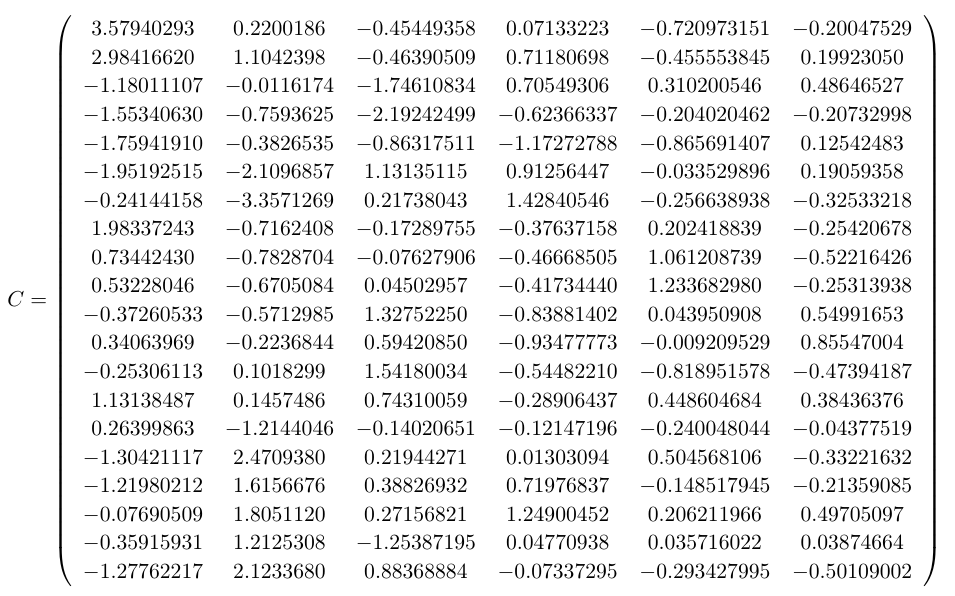
\includegraphics[width=12cm]{imagenes/C.png}
        \label{figura1}
    \end{center}
\end{figure}
}
\end{frame}

\begin{frame}
\frametitle{ACP para los individuos $R^6$}
\Wider[4em]{
\begin{figure}[h]
  \centering
  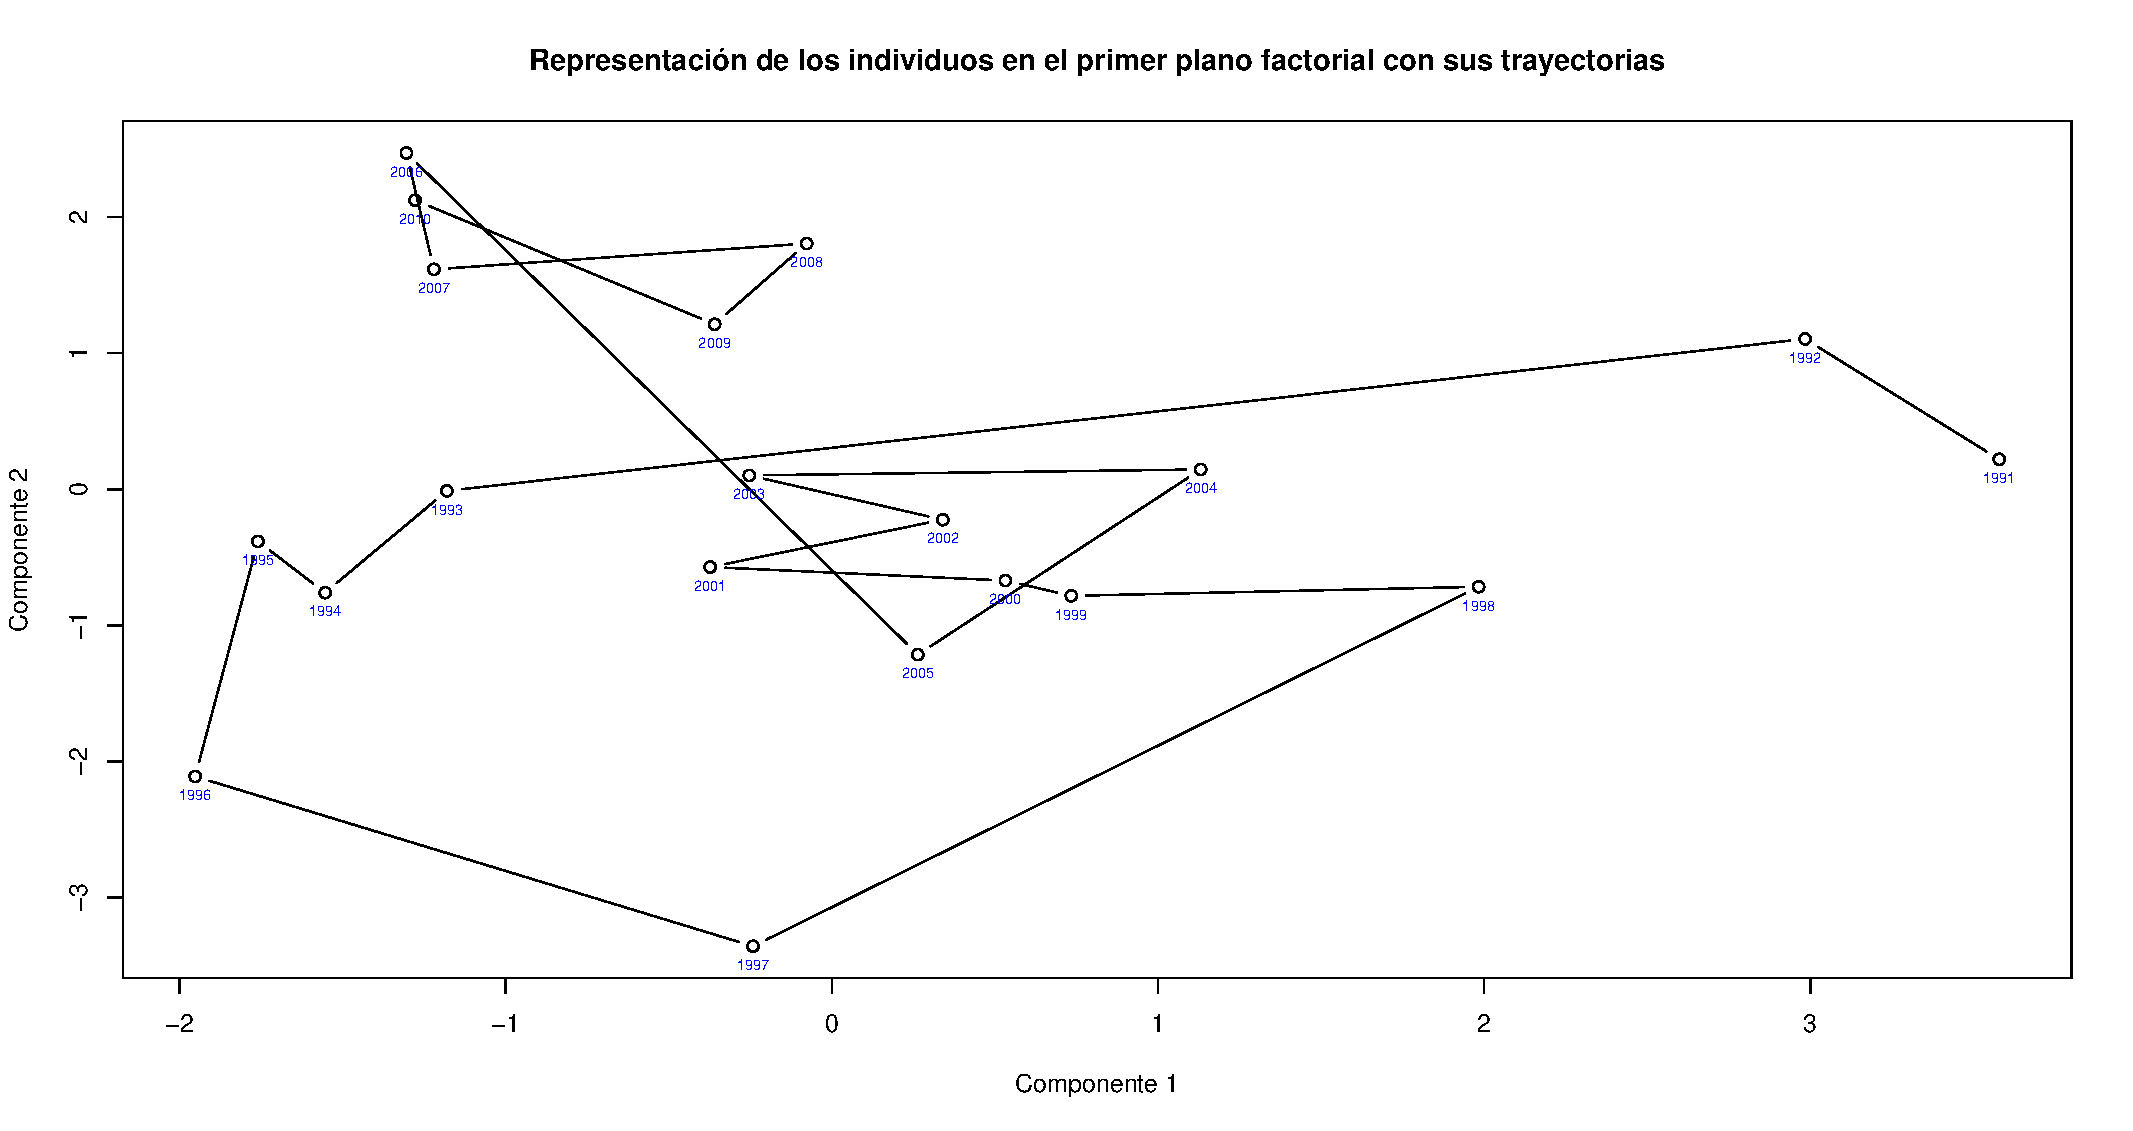
\includegraphics[scale=0.35]{imagenes/1.pdf}
  \caption{Representación de los individuos}\label{figura1}
\end{figure}
}
\end{frame}

\begin{frame}
\frametitle{ACP para los individuos $R^6$}
~\\En la figura 1 podemos ver claramente como la línea entre 1991 y 1992 es corta, esto porque los promedios de importaciones en esos 2 años fueron muy cercanos, mientras que un año después, la línea entre 1992 y 1993, es mucho más larga y esto es porque el año de 1993 tuvo un promedio de importaciones de 90.78333 mientras que en 1992 el promedio de importaciones fue solo de 33.5; basados en esto podemos decir que entre los años 1995 y 1999 las importaciones en los países suramericanos tuvieron un crecimiento mayor al de los años anteriores, mientras que en los años siguientes su crecimiento fue mas constante.
\end{frame}

\begin{frame}
\frametitle{ACP para los individuos $R^6$}
~\\Para decidir cuantas componentes principales utilizar, nos centramos en el criterio de los valores propios, el cuál nos dice que debemos utilizar las componentes cuyo valor propio sea mayor a la unidad. Para decidir esto, realizamos la siguiente tabla y la siguiente gráfica para tener en cuenta también, el porcentaje de inercia acumulado entre las componentes que vayamos a seleccionar.

\begin{center}
\begin{tabular}{|c|c|c|c|}
\hline 
 & Valor propio & Porcentaje de Inercia & Inercia Acumulada \\ 
\hline 
$\lambda_1$ & 2.1934092 & $36.56 \%$ & $36.56 \%$ \\ 
$\lambda_2$ & 1.9561781 & $32.60 \%$ & $69.16 \%$ \\  
$\lambda_3$ & 0.9038789 & $15.06 \%$ & $84.22 \%$ \\ 
$\lambda_4$ & 0.5119470 & $8.53 \%$ & $92.75 \%$ \\ 
$\lambda_5$ & 0.2854407 & $4.76 \%$ & $97.51 \%$ \\  
$\lambda_6$ & 0.1491461 & $2.49 \%$ & $100 \% $ \\ 
\hline 
\end{tabular} 
\end{center}
\end{frame}

\begin{frame}
\frametitle{ACP para los individuos $R^6$}
\begin{figure}[h]
  \centering
  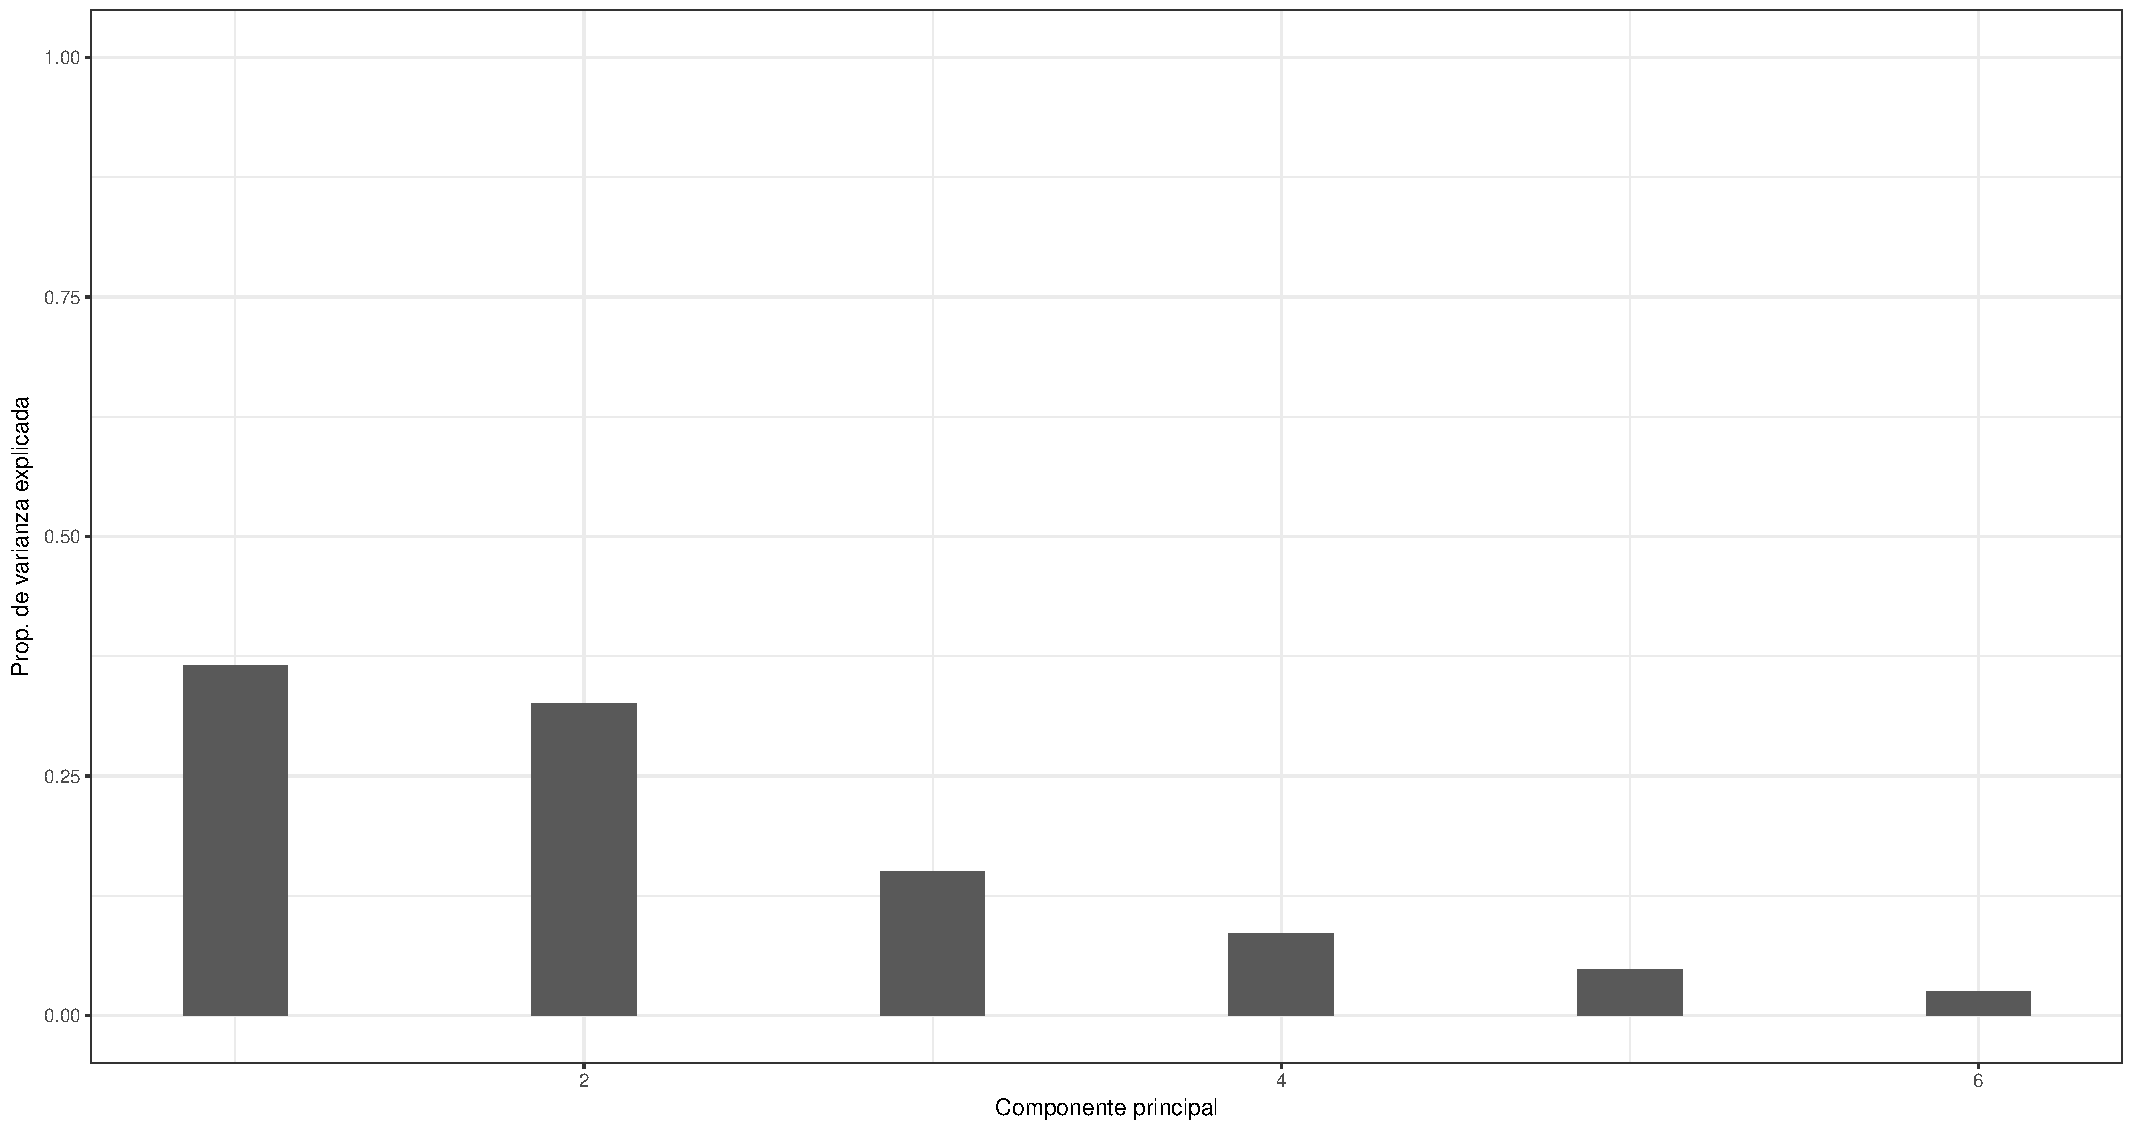
\includegraphics[scale=0.32]{imagenes/varexp.pdf}
  \caption{Gráfico de barras de la inercia explicada por las componentes principales}\label{figura1}
\end{figure}
\end{frame}

\begin{frame}
\frametitle{ACP para los individuos $R^6$}
~\\De acuerdo a lo anterior, seleccionamos las primeras dos componentes principales, ya que sus valores propios correspondientes son los únicos mayor a la unidad y además, el porcentaje de inercia acumulado entre ellas dos es de casi el $70\%$.
\end{frame}

\begin{frame}
\frametitle{ACP para los individuos $R^6$}
\begin{figure}[h]
  \centering
  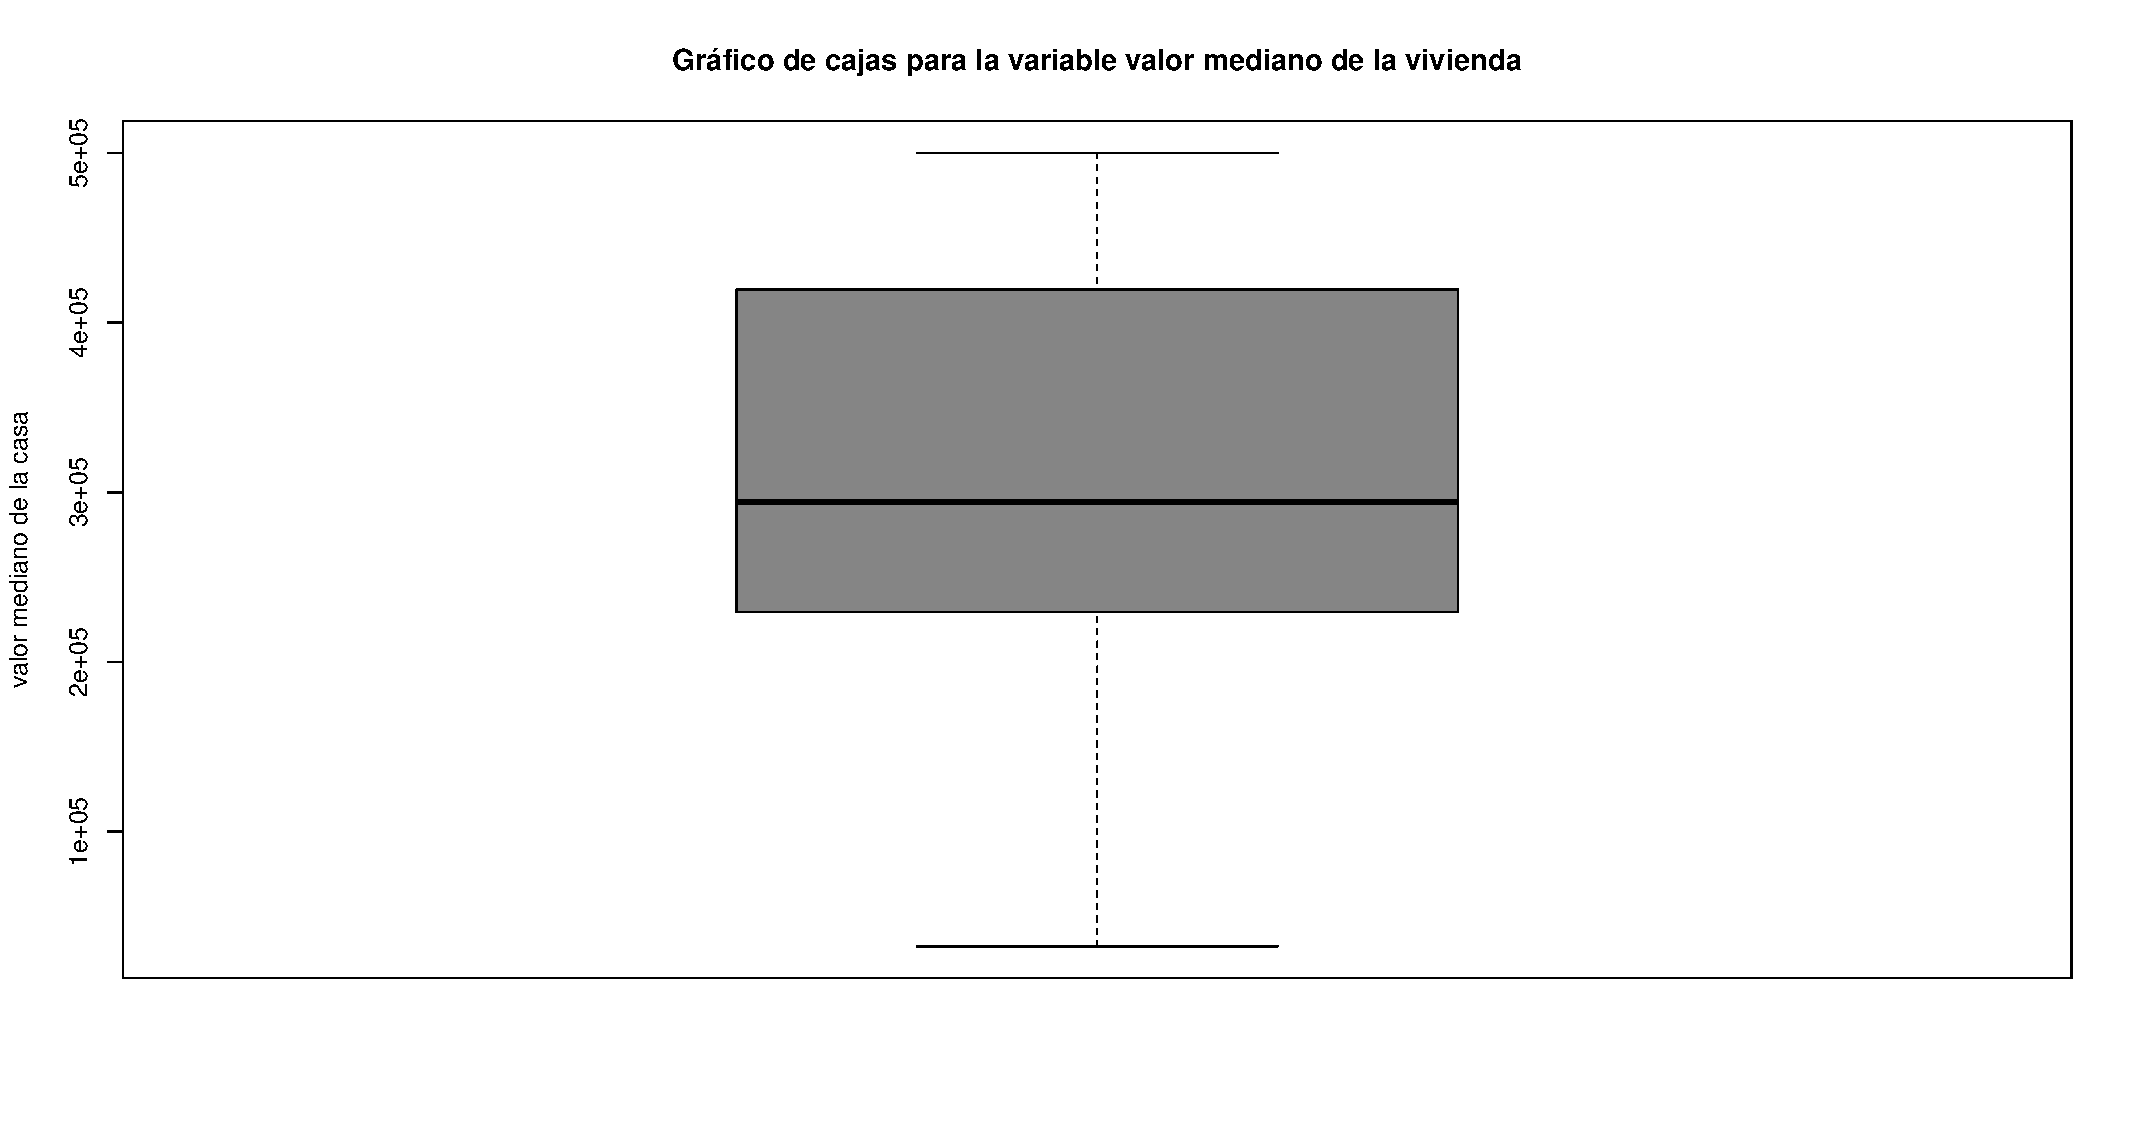
\includegraphics[scale=0.32]{imagenes/2.pdf}
  \caption{Círculo de correlaciones para las variables de la tabla de importaciones generado por las dos
primeras componentes principales}\label{figura1}
\end{figure}
\end{frame}

\begin{frame}
\frametitle{ACP para los individuos $R^6$}
~\\En esta gráfica se puede observar que las variables mejor representadas por el plano son los países Colombia y Perú, ya que la recta esta más cerca del limite del circulo de correlaciones, esto nos dice que estas dos variables tienen una correlación elevada con las componentes que generan el plano. Los países Brasil, Chile y Ecuador también son bien representados, pero no tanto como los dos primeros. Argentina tiene poca representación en el plano formado.
\end{frame}

\begin{frame}
\frametitle{ACP para los individuos $R^6$}
\begin{figure}[h!]
  \centering
  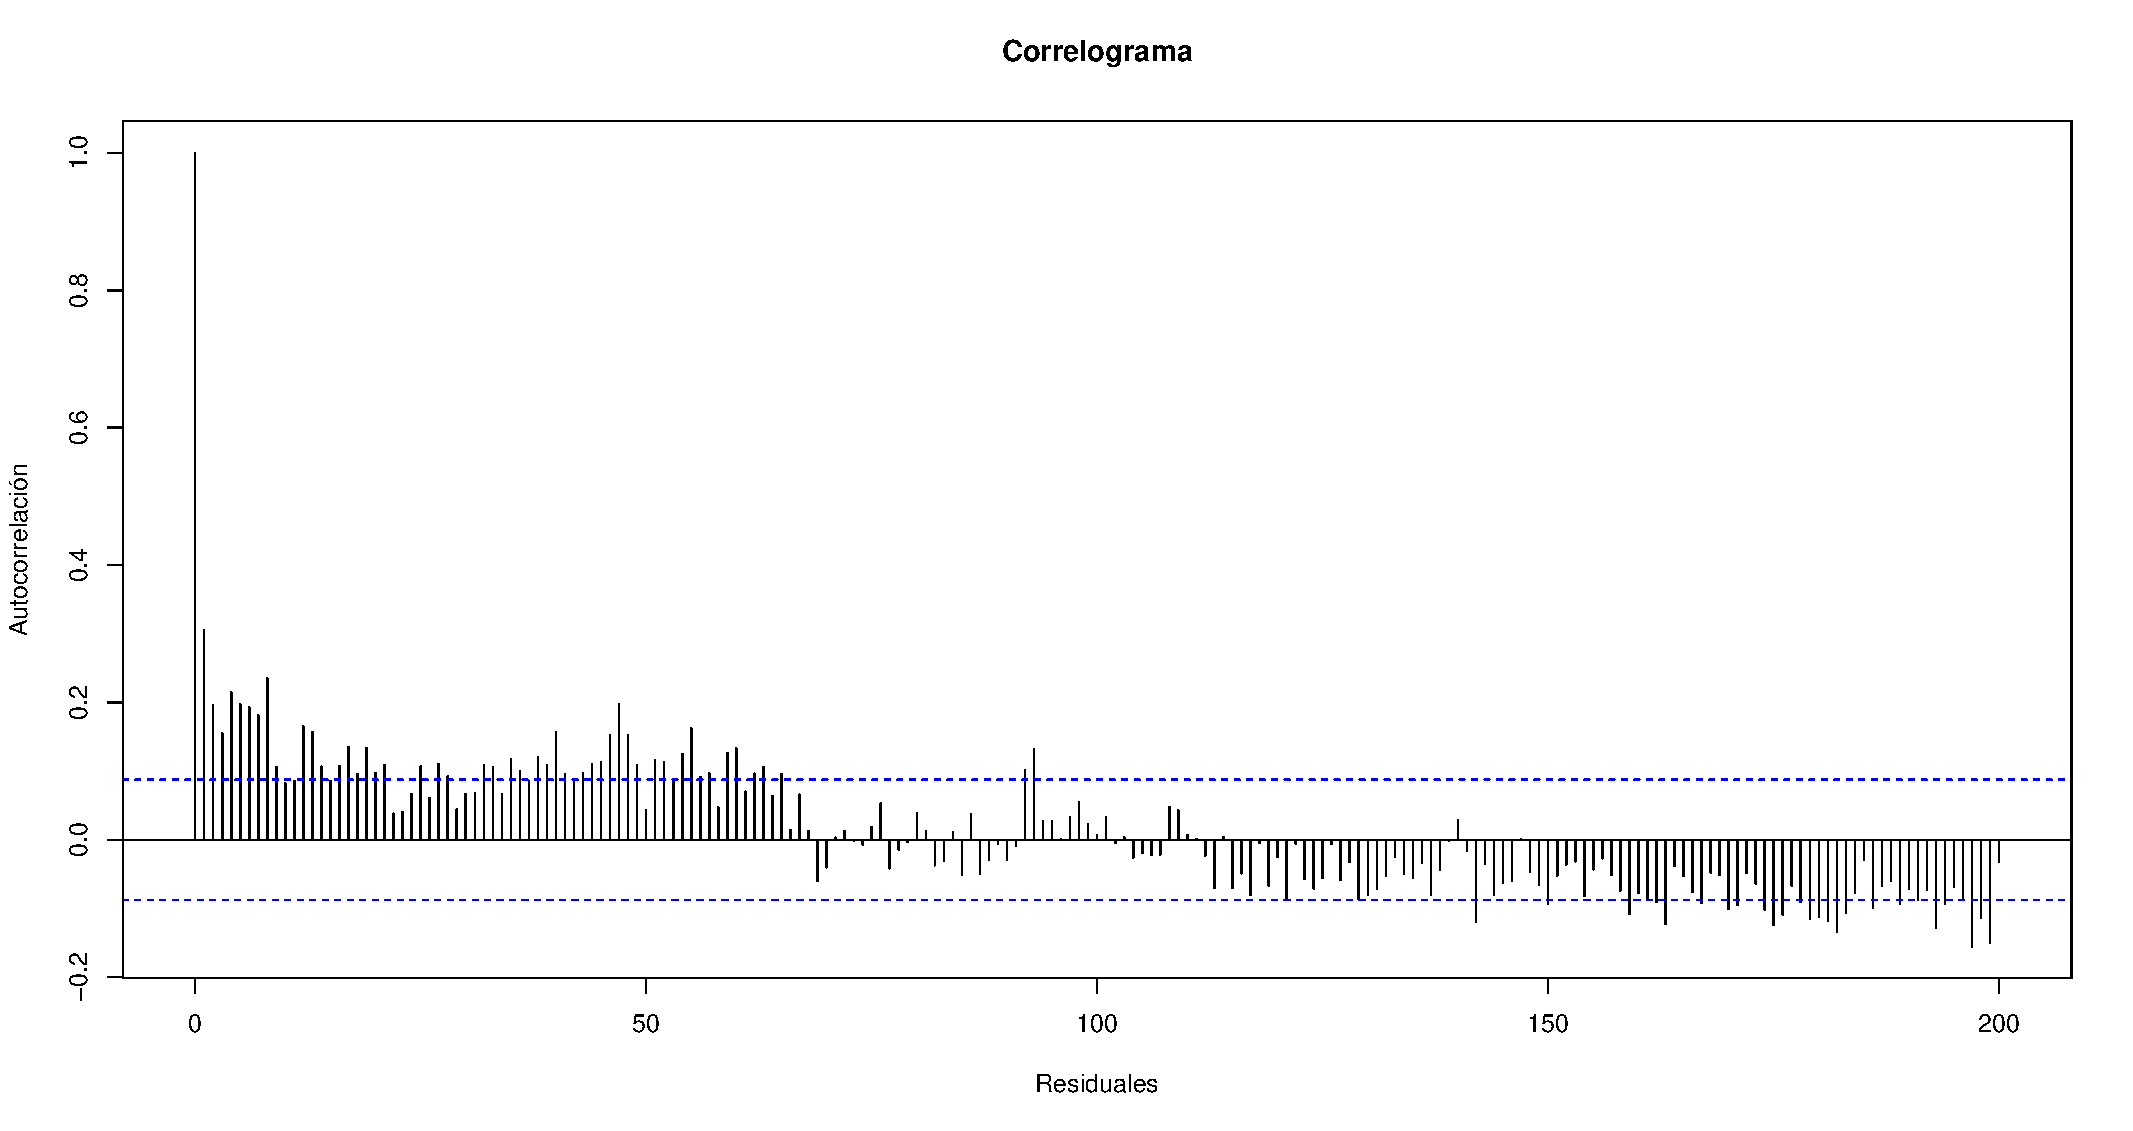
\includegraphics[scale=0.32]{imagenes/4.pdf}
  \caption{Representación de los individuos}\label{figura1}
\end{figure}
\end{frame}

\begin{frame}
\frametitle{ACP para los individuos $R^6$}
\begin{figure}[h]
  \centering
  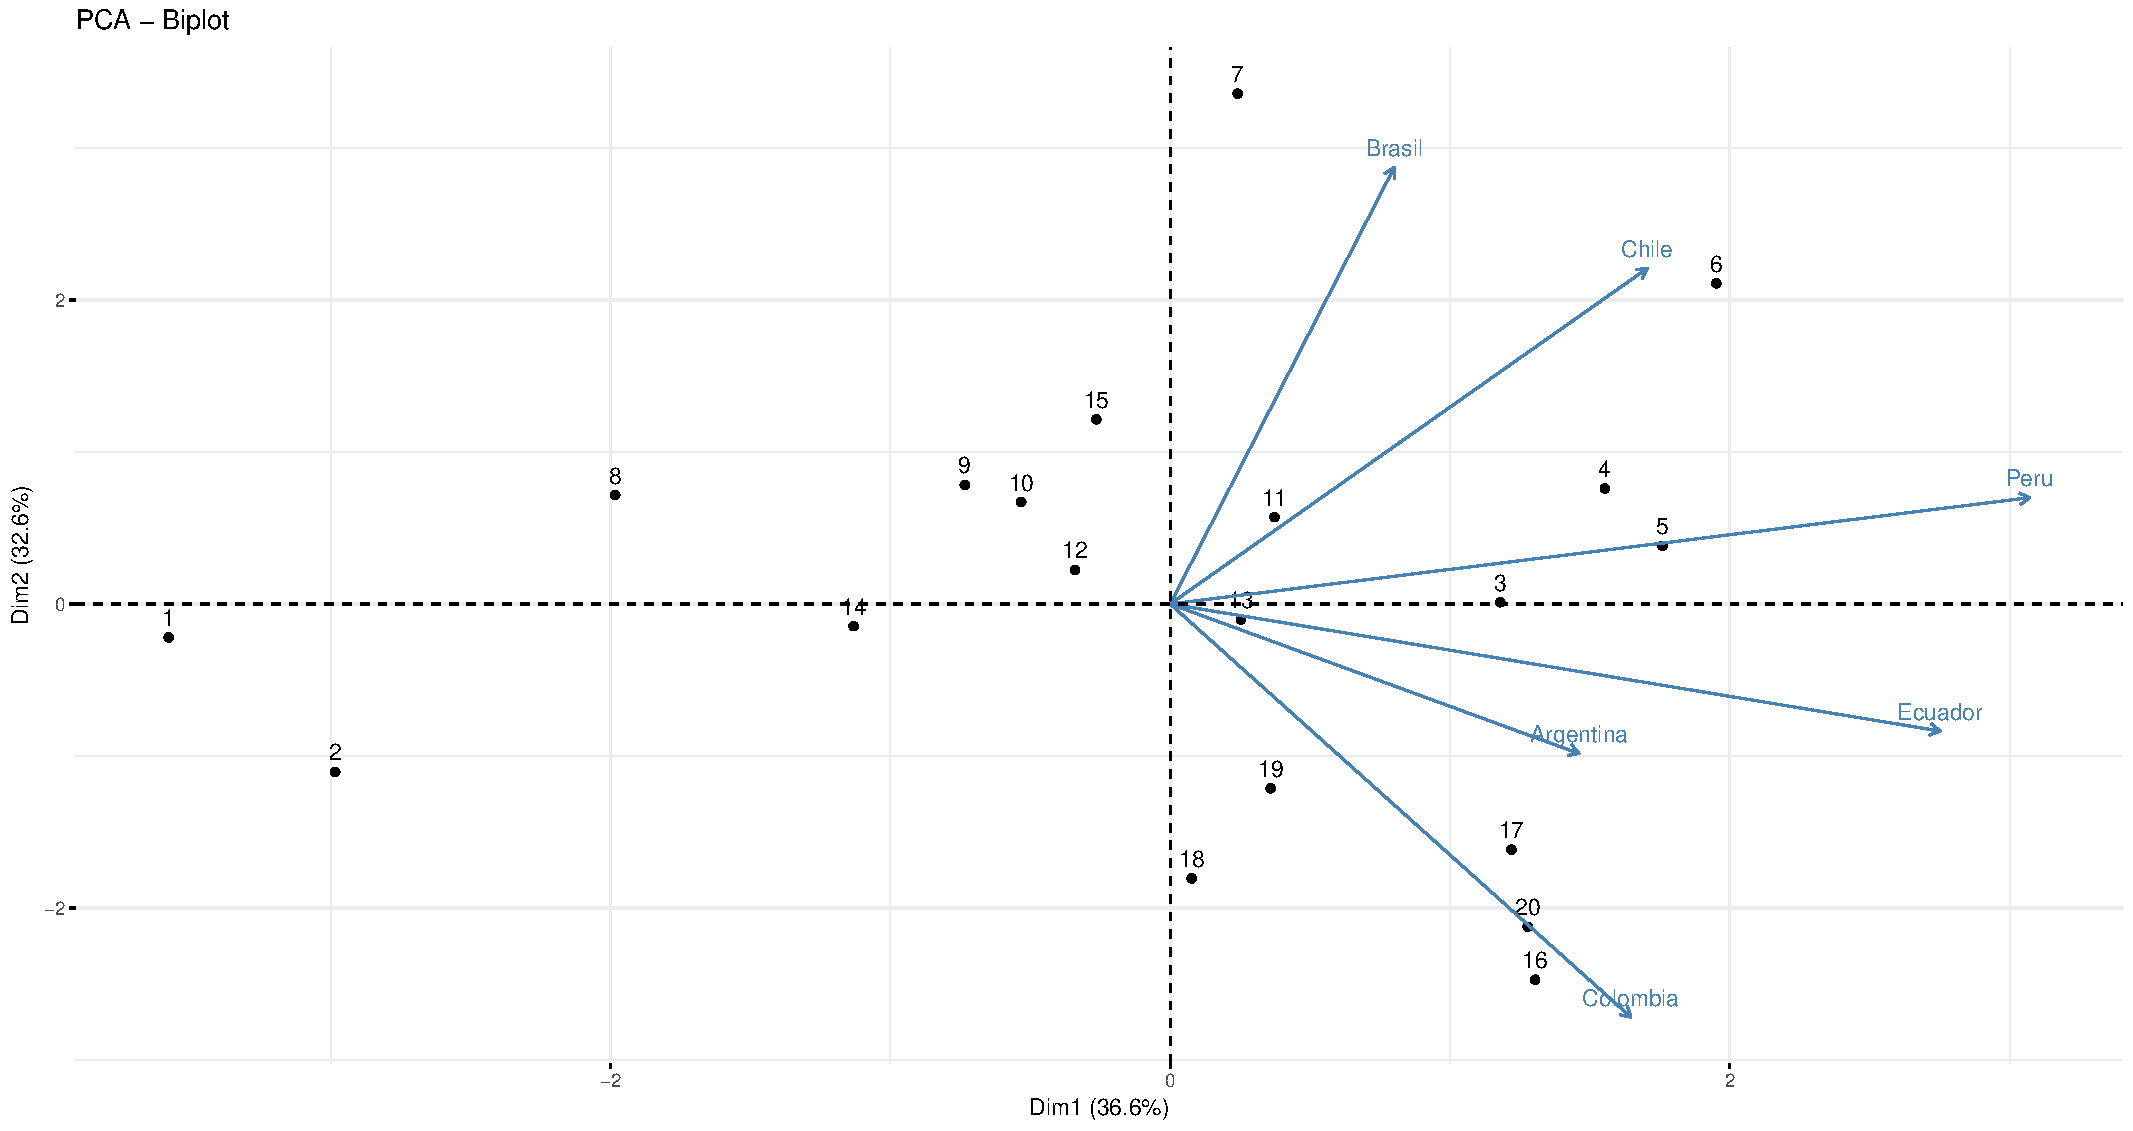
\includegraphics[scale=0.32]{imagenes/5.pdf}
  \caption{Primer plano principal para la tabla de importaciones, generado por las dos
primeras componentes principales}\label{figura1}
\end{figure}
\end{frame}

\begin{frame}
\frametitle{ACP para los individuos $R^6$}
~\\En la figura 5 podemos ver los vectores correspondientes a cada variable (país), de los cuales podemos notar que países como: Perú, Ecuador y Argentina tienen alta correlación con el eje 1, por ende, años con valores altos en la componente 1 significan altas importaciones en dichos países y valores bajos en la componente 1 significan bajas importaciones en dichos países en esos años, por otra parte; Colombia y Chile tiene una correlación intermedia, ósea el ángulo que forma el vector entre la variable y el eje 1 es similar al ángulo que forma la variable con el eje 2, por tanto, valores altos en los dos ejes significa altas importaciones para Chile en ese año y valores bajos en ambos ejes, significan altas importaciones para Colombia. Por otra parte, Brasil tiene alta correlación con el eje 2, por ende, valores altos en la componente 2 significan altas importaciones esos años en Brasil.
\end{frame}

\begin{frame}
\frametitle{ACP para los individuos $R^6$}
\Wider[1em]{
~\\Los cosenos cuadrados y las contribuciones en las dos primeras dimensiones para los individuos son:
\begin{center}
\resizebox{6.5cm}{!}{
\begin{tabular}{|cc|cc|}
\hline 
 Cosenos & Cuadrados  & Contribuciones  &   \\ 
Componente 1 & Componente 2 & Componente 1 & Componente 2 \\ 
0.939844281 & 0.003551024 & 29.20596190 & 0.1237316 \\ 
0.802730728 & 0.1099134 & 20.30001454 & 3.116652 \\  
0.264147747 & 0.0000256 & 3.17465182 & 0.00034497 \\ 
0.291786249 & 0.06972573 & 5.50073162 & 1.473873 \\ 
0.505191102 & 0.02389618 & 7.05649339 & 0.3742597 \\  
0.365961449 & 0.4275083 & 8.68513660 & 11.37620 \\ 
0.004290144 & 0.8294368 & 0.13288454 & 28.80694 \\
0.832735084 & 0.1085967 & 8.96724173 & 1.311233 \\
0.194391979 & 0.2208839 & 1.22954496 & 1.566540 \\
0.113548769 & 0.1801813 & 0.64584957 & 1.149132 \\
0.042910068 & 0.1008759 & 0.31648160 & 0.8342337 \\
0.054608053 & 0.02354711 & 0.26450923 & 0.1278890 \\
0.017575565 & 0.0028458 & 0.14598264 & 0.02650405 \\
0.559940767 & 0.00929244 & 2.91790445 & 0.05429631 \\
0.042537936 & 0.9001189 & 0.15887431 & 3.769540 \\
0.206935729 & 0.7427854 & 3.87744963 & 15.60577 \\
0.307751740 & 0.5399155 & 3.39179115 & 6.672147 \\
0.001140083 & 0.6281081 & 0.01348219 & 8.328560 \\
0.040609619 & 0.4628499 & 0.29405231 & 3.757917 \\
0.224698257 & 0.6206480 & 3.72096180 & 11.52424 \\
\hline 
\end{tabular} 
}
\end{center}
}
\end{frame}

\begin{frame}
\frametitle{ACP para los individuos $R^6$}
~\\Con respecto a la tabla anterior, podemos observar que los cosenos cuadrados del primero, segundo, quinto, octavo,y catorceavo año (1991,1992, 1995, 1998 y 2004 respectivamente) son los más altos con 0.94,0.80,0.50,0.83 y 0.56 respectivamente, en la primera componente principal. Esto nos dice que dichos individuos en este caso, esos años, están muy bien representados en el plano principal. En cuanto a la segunda componente principal, están mejor representados en el plano principal los años 1997,2005, 2006, 2007, 2008, 2009 y 2010, ya que son los años que tienen mayor cosenos cuadrados.
\end{frame}

\begin{frame}
\frametitle{ACP para los individuos $R^6$}
~\\Ahora, en cuanto a las contribuciones de los individuos, podemos notar que los años 1991, 1992, 1996 y 1998 son los que más aporte tuvieron en la construcción del eje 1, ya que sus contribuciones son las más altas. Los años 1996, 1997, 2006, 2008 y 2010 tuvieron un aporte alto en la construcción del eje 2 por sus valores altos en las contribuciones.
\end{frame}

\begin{frame}
\frametitle{ACP para las variables $R^{20}$}
~\\Para realizar el análisis de componentes principales en el espacio de las variables ($R^20$) ya no hacemos uso de la matriz de correlaciones para la descomposición en valores y vectores propios. 

~\\Construimos la matriz $N^{\frac{1}{2}}ZZ'N^{\frac{1}{2}}$ donde N es una matriz $nxn$ diagonal de métricas (en nuestro caso es diagonal de $\frac{1}{20}$) y Z es la matriz de datos estandarizada.

~\\Omitiremos parte de esta matriz por ser de dimensión 20x20, mostraremos las primeras 6 columnas
\end{frame}

\begin{frame}
\frametitle{ACP para las variables $R^{20}$}
\Wider[4em]{
\begin{figure}[!h]
    \begin{center}
        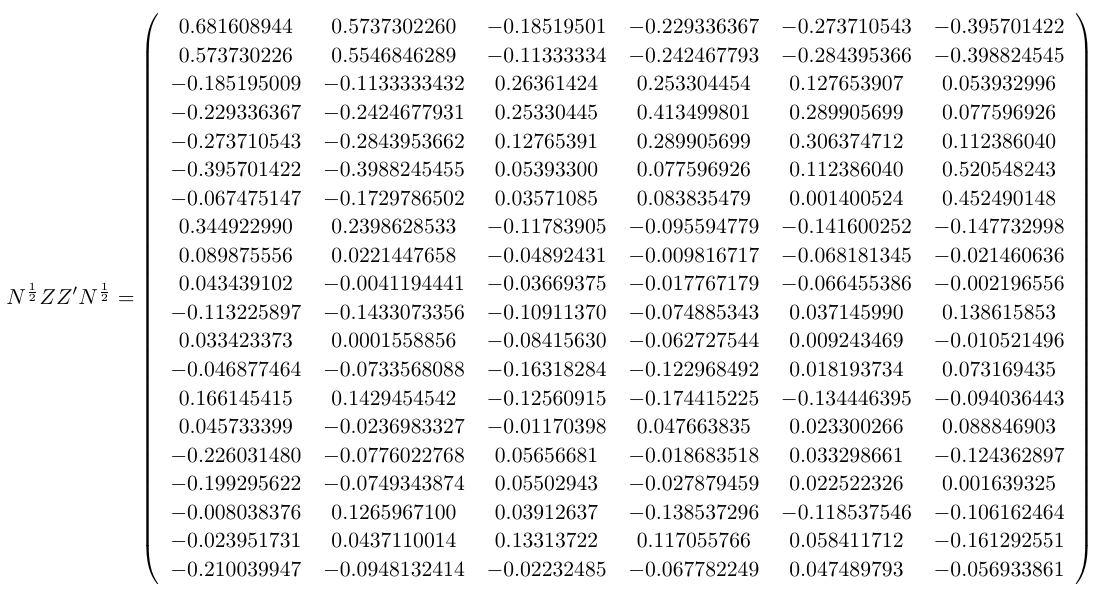
\includegraphics[width=12.5cm]{imagenes/N.png}
        \label{figura1}
    \end{center}
\end{figure}
}
\end{frame}

\begin{frame}
\frametitle{ACP para las variables $R^{20}$}
~\\Ahora, en este caso, se debe descomponer en valores y vectores propios la matriz anterior.

~\\Los valores propios son: $\lambda_1=2.193409$,  $\lambda_2=1.956178$,$\lambda_3= 0.9038789$, $\lambda_4=0.5119470$, $\lambda_5=0.2854407$,$\lambda_6=0.1491461$ , $\lambda_i=0$ $i=7,\cdots,20$.

~\\Y, de los 20 vectores propios asociados solo se mostrarán los primeros 6.
\end{frame}

\begin{frame}
\frametitle{ACP para las variables $R^{20}$}
\begin{center}
\resizebox{11cm}{!}{
\begin{tabular}{|cccccc|}
\hline 
$\lambda_{1}$ & $\lambda_{2}$ & $\lambda_{3}$ & $\lambda_{4}$ & $\lambda_{5}$ & $\lambda_{6}$ \\ 
-0.54042541& -0.035175496& -0.10689506& -0.02229248&  0.301749219&  0.11607531 \\ 
-0.45055537& -0.176540432& -0.10910861& -0.22245121&  0.190663157& -0.11535458 \\ 
0.17817553&  0.001857333& -0.41067765& -0.22047800& -0.129828375& -0.28166368 \\ 
0.23453639&  0.121403156& -0.51564953&  0.19490490&  0.085388776&  0.12004418 \\ 
0.26564061&  0.061176767& -0.20301531&  0.36649645&  0.362318216& -0.07262105 \\ 
0.29470556&  0.337286185&  0.26608924& -0.28519117&  0.014033283& -0.11035380 \\ 
0.03645333&  0.536720974&  0.05112700& -0.44639983&  0.107411211&  0.18836753 \\
-0.29945353&  0.114509067& -0.04066481&  0.11762221& -0.084718448&  0.14718587 \\
-0.11088485&  0.125161482& -0.01794053&  0.14584663& -0.444148173&  0.30233342 \\
-0.08036477&  0.107197588&  0.01059077&  0.13042688& -0.516333895&  0.14656785 \\
0.05625670&  0.091336397&  0.31222795&  0.26214296& -0.018394793& -0.31840200 \\
-0.05143046&  0.035761568&  0.13975545&  0.29213317&  0.003854469& -0.49531767 \\
0.03820767& -0.016280064&  0.36262524&  0.17026573&  0.342756174&  0.27441262 \\
-0.17081875& -0.023301569&  0.17477427&  0.09033730& -0.187754721& -0.22254684 \\
-0.03985904&  0.194153041& -0.03297601&  0.03796196&  0.100467416&  0.02534586 \\
0.19691241& -0.395041436&  0.05161204& -0.00407238& -0.211177117&  0.19235345 \\
0.18416816& -0.258304997&  0.09131938& -0.22493927&  0.062159283&  0.12366923 \\
0.01161128& -0.288592444&  0.06387175& -0.39033413& -0.086305988& -0.28779281 \\
0.05422659& -0.193853472& -0.29490564& -0.01490995& -0.014948243& -0.02243433 \\
0.19289795& -0.339473648&  0.20784006&  0.02293024&  0.122808551&  0.29013142 \\
\hline 
\end{tabular} 
}
\end{center}
\end{frame}

\begin{frame}
\frametitle{ACP para las variables $R^{20}$}
~\\Ahora, para encontrar finalmente las componentes principales, hacemos el producto:
$$Z'N^{\frac{1}{2}}V$$

~\\Las 6 primeras componentes principales están dadas por:
\begin{center}
\resizebox{12cm}{!}{
\begin{tabular}{|ccccccc|}
\hline 
País & $C_1$ & $C_2$ & $C_3$ & $C_4$ & $C_5$ & $C_6$ \\ 
Colombia & 0.4837847& -0.7984781&  0.006466285& -0.08377667& -0.28489471& -0.20039902 \\ 
Brasil & 0.2352724&  0.8438349&  0.191084241&  0.38735334& -0.09898461& -0.19035719 \\ 
Chile & 0.5008368&  0.6484013&  0.048892549& -0.56456896&  0.04162357& -0.07666214 \\ 
Argentina & 0.4292863& -0.2889960&  0.842721906&  0.03210461&  0.13121512&  0.06136957 \\ 
Ecuador & 0.8085448& -0.2456063& -0.359939262&  0.15857133&  0.35401184& -0.07685944 \\ 
Peru & 0.9028508&  0.2056407& -0.158735325&  0.09986052& -0.22406122&  0.23916484 \\ 
\hline 
\end{tabular} 
}
\end{center}
\end{frame}

\begin{frame}
\frametitle{ACP para las variables $R^{20}$}
\begin{figure}[h]
  \centering
  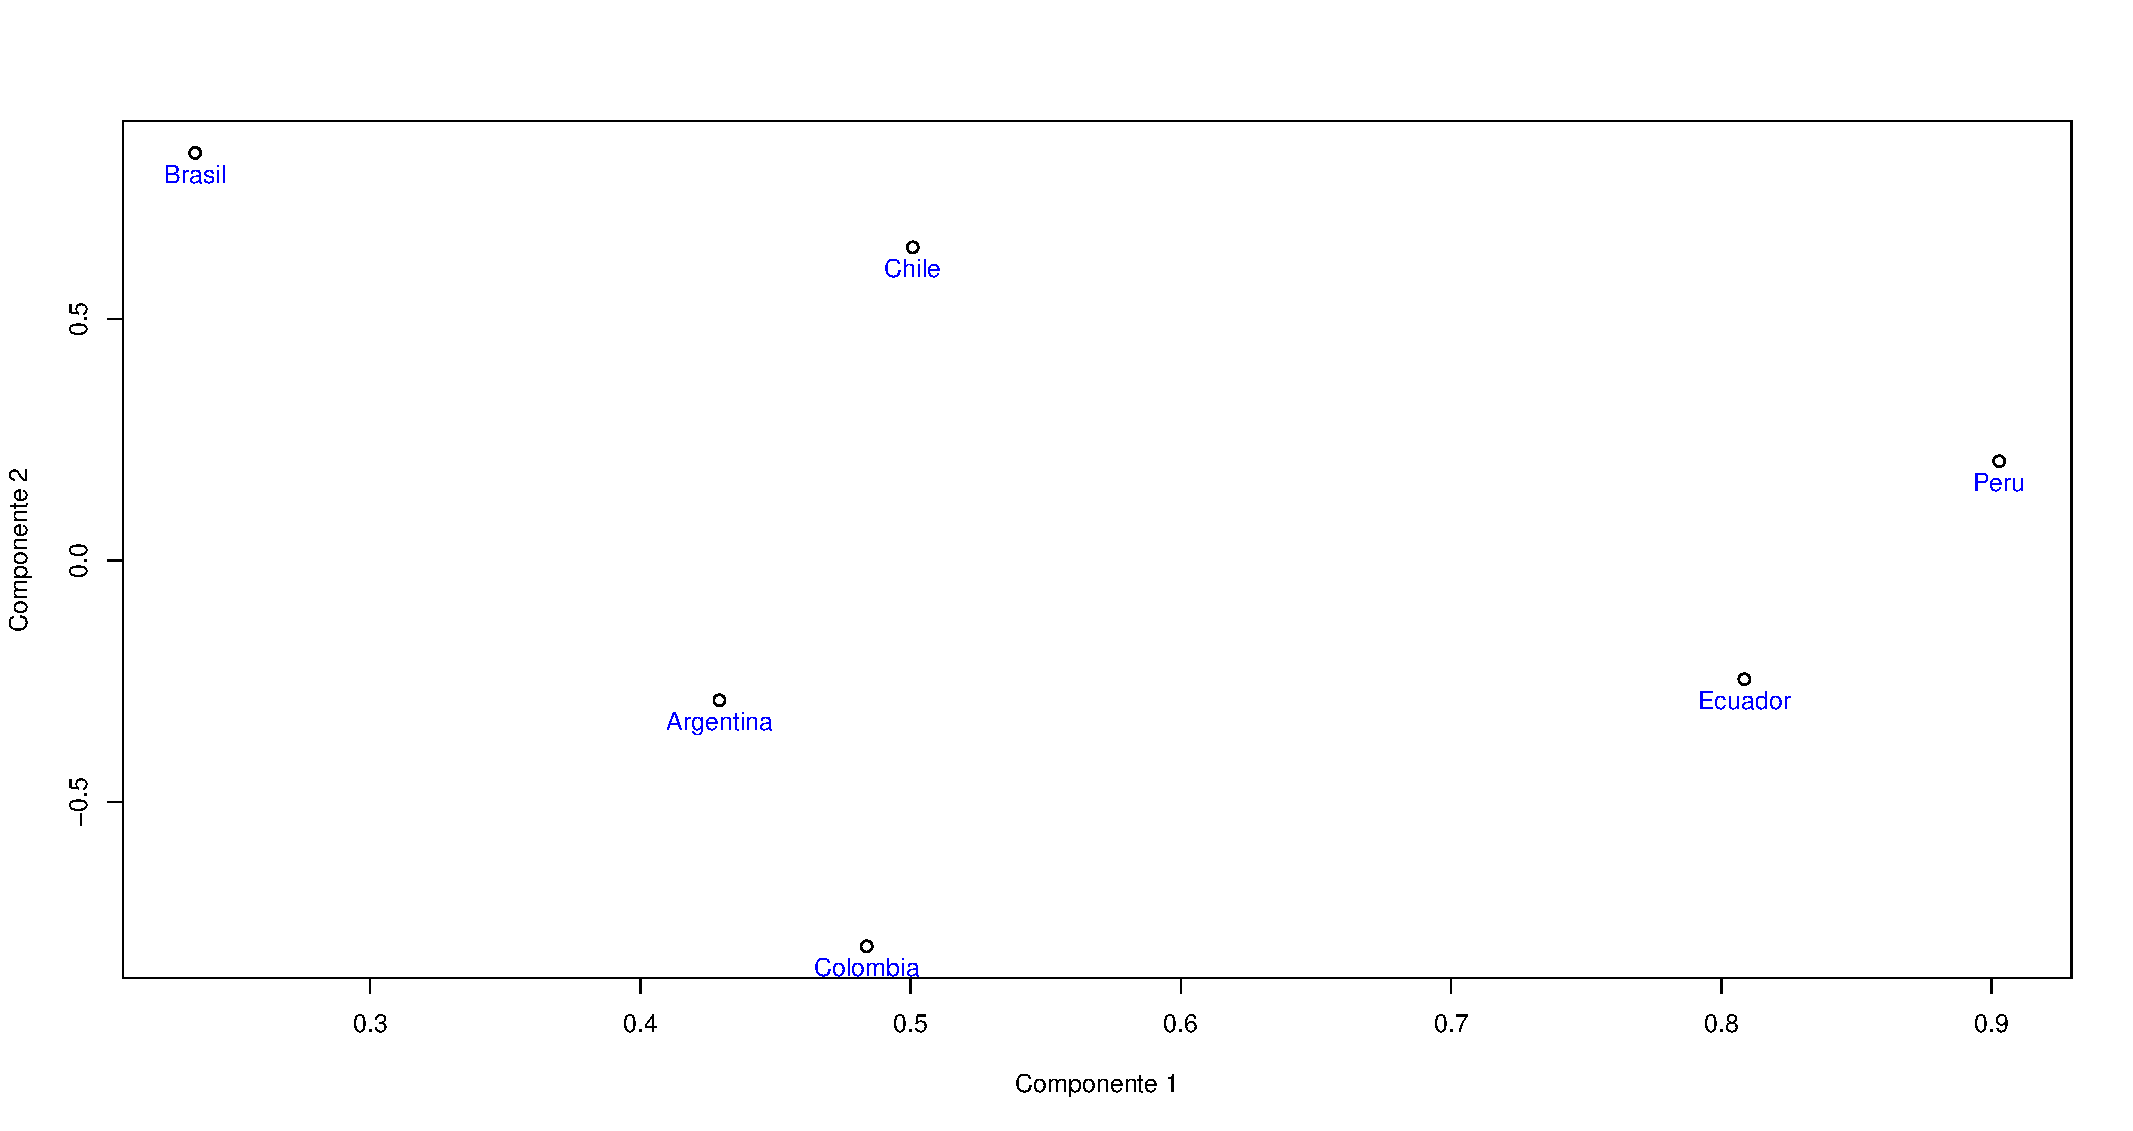
\includegraphics[scale=0.33]{imagenes/6.pdf}
  \caption{Representación de las variables}\label{figura1}
\end{figure}
\end{frame}

\begin{frame}
\frametitle{ACP para las variables $R^{20}$}
~\\Los cosenos cuadrados y las contribuciones en las dos primeras dimensiones para las variables son:
\begin{center}
\resizebox{12cm}{!}{
\begin{tabular}{|c|cc|cc|}
\hline 
 País &Cosenos &Cuadrados  & contribuciones  &   \\ 
 &Componente 1 & Componente 2 & Componente 1 & Componente 2 \\ 
Colombia &0.23404762 & 0.63756727 & 10.670495 & 32.592496 \\ 
Brasil &0.05535309 &0.71205730 & 2.523610 & 36.400433 \\  
Chile &0.25083751 &0.42042429 & 11.435965 & 21.492127 \\ 
Argentina &0.18428677 &0.08351869 & 8.401841 & 4.269483 \\ 
Ecuador &0.65374465 & 0.06032246 & 29.804956 & 3.083689 \\  
Peru &0.81513961 & 0.04228811 & 37.163134 & 2.161772 \\ 
\hline 
\end{tabular} 
}
\end{center}
\end{frame}

\begin{frame}
\frametitle{ACP para las variables $R^{20}$}
~\\Con respecto a la tabla anterior, podemos observar que los cosenos cuadrados de los países Ecuador y Perú son los más altos con 0.6537 y 0.8151 respectivamente, en la primera componente principal. Esto nos dice que dichas variables en este caso, estos países, están muy bien representados en el plano principal correspondiente  a las variables. En cuanto a la segunda componente principal, están mejor representados en el plano principal los países Colombia, Brasil y un poco Chile. El país Argentina se encuentra muy bien representado (con $cos^2=0.71$) en la tercera componente que no fue expuesta en la tabla.
\end{frame}

\begin{frame}
\frametitle{ACP para las variables $R^{20}$}
~\\Ahora, en cuanto a las contribuciones de las variables, podemos notar que los países Perú, Ecuador, Chile y Colombia son los que más aporte tuvieron en la construcción del eje 1, ya que sus contribuciones son las más altas. En cuanto a la construcción del eje 2, los países que mas contribuyeron fueron Brasil, Colombia y Chile.
\end{frame}

\begin{frame}
\frametitle{Construcción de Indice}
~\\En las componentes principales correspondientes al ACP para las variables, podemos observar que la primera componente tiene todos los valores positivos, esto nos dice que todos los 6 países están relacionados positivamente con el eje 1, por lo cuál tenemos lo que se llama factor tamaño y se puede construir un indice con dicha componente de la siguiente manera:
$$I=0.4837847 Colombia+0.2352724 Brasil + 0.5008368 Chile$$ 
$$+0.4292863 Argentina+0.8085448 Ecuador+0.9028508 Peru$$
\end{frame}

\begin{frame}
\frametitle{Construcción de Indice}
~\\INDICE DEL CRECIMIENTO ECONÓMICO EN SUDAMÉRICA:
~\\Los betas o coeficientes en la regresión anterior nos indican la correlación de la variable con nuestro índice, esto se podría interpretar también como la importancia del país dentro del crecimiento económico en Sudamérica. Con el modelo dado anteriormente, tendremos 20 indices (uno para cada año) de crecimiento económico en Sudamérica.

~\\En la siguiente tabla se mostraran los 20 indices originales arrojados por el modelo de la primera componente principal, pero además, se mostrarán los indices re escalados a una escala de 0 a 100, donde 0 no implica la ausencia del crecimiento y económico, simplemente significa que fue el menor indice que se obtuvo y 100 significa que ese fue el indice más alto que se obtuvo.
\end{frame}

\begin{frame}
\frametitle{Construcción de Indice}
~\\La transformación que se utilizó para re escalar los indices originales fue la siguiente:
$$\left(\frac{I-\min{I}}{\max{I}-\min{I}}\right)\cdot 100$$
\end{frame}

\begin{frame}
\frametitle{Construcción de Indice}
\Wider[4em]{
\begin{center}
\resizebox{5.5cm}{!}{
\begin{tabular}{|c|c|c|}
\hline 
Año & Indice Original & Indice re-escalado \\ 
\hline 
1991 & 76.8848 & 0 \\ 
1992 & 105.8963 & 9.886876 \\ 
1993 & 340.6289 & 89.88188 \\  
1994 & 370.3189 & 100 \\  
1995 & 370.202 & 99.96016 \\  
1996 & 351.938 & 93.73593 \\ 
1997 & 274.2018 & 67.24405 \\ 
1998 & 153.4388 & 26.08901 \\  
1999 & 212.3041 & 46.1498 \\  
2000 & 220.6235 & 48.98501 \\  
2001 & 263.5299 & 63.60716 \\  
2002 & 234.8063 & 53.81839 \\  
2003 & 257.935 & 61.70048 \\  
2004 & 185.6864 & 37.07872 \\  
2005 & 249.2168 & 58.72936 \\  
2006 & 316.7728 & 81.75191 \\  
2007 & 316.2897 & 81.58728 \\ 
2008 & 254.7682 & 60.62123 \\  
2009 & 290.352 & 72.74792 \\  
2010 & 313.4227 & 80.61023 \\ 
\hline 
\end{tabular}
} 
\end{center}
}
\end{frame}

\begin{frame}
\frametitle{Construcción de Indice}
~\\Con los indices construidos y observando la tabla anterior, podemos concluir que el año que menos crecimiento económico hubo en Sudamérica fue en 1991, y los años en los cuales hubo un crecimiento económico notable fueron en 1993,1995,1996 y 1994. Si vemos la base de datos original, podemos observar que justamente en el año 1991 fue donde menos importaciones tuvieron los países en general, en cambio, si observamos el año 1994, que corresponde a 100 en la escala nueva, fue el año en el cual se tuvo un gran número de importaciones para todos los países.
\end{frame}

\begin{frame}
\frametitle{Referencias}
\begin{itemize}
\item Kassambara, A. \& Mundt, F. (2017), factoextra: Extract and Visualize the Results of Multivariate
Data Analyses. R package version 1.0.5.
*https://CRAN.R-project.org/package=factoextra


\item Lê, S., Josse, J. \& Husson, F. (2008), 'FactoMineR: A package for multivariate analysis', Journal
of Statistical Software 25(1), 1-18.


\item Ludovic Lebart, Alain Morineau, M. P. (1995), Statistique exploratoire multidimensionnelle, Dunod,
Paris.
\end{itemize}
\end{frame}

\begin{frame}
\frametitle{Referencias}
\begin{itemize}
\item Wickham, H. (2009), ggplot2: Elegant Graphics for Data Analysis, Springer-Verlag New York.
*http://ggplot2.org


\item Wickham, H. \& Bryan, J. (2018), readxl: Read Excel Files. R package version 1.1.0.
*https://CRAN.R-project.org/package=readxl


\item Zelaya, J. T. (n.d.), ANÁLISIS MULTIVARIADO DE DATOS, Universidad de Costa Rica.
\end{itemize}
\end{frame}

\end{document}